\section{Algebra}

\subsection{Vektoren}

\boxx{Form}{
    \begin{equation*}
        \vec{AB}\begin{pmatrix}
            b_1-a1\\
            b_2-a_2\\
            b_3-a_3
        \end{pmatrix}
    \end{equation*}
}

\boxx{Vektoren Addieren \& Subtrahieren}{
    \begin{center}
        Addition:
    \end{center}
    \begin{equation*}
        \vec{a}+\vec{b}=\begin{pmatrix}
            a_1+b_1\\
            a_2+b_2\\
            a_3+b_3
        \end{pmatrix}
    \end{equation*}
    \begin{center}
        Subtraktion:
    \end{center}
    \begin{equation*}
        \vec{a}-\vec{b}=\begin{pmatrix}
            a_1-b_1\\
            a_2-b_2\\
            a_3-b_3
        \end{pmatrix}
    \end{equation*}
}

\boxx{Betrag eines Vektors}{
    \begin{equation*}
        |\vec{a}|=\sqrt{a_1^2+a_2^2+a_3^2}
    \end{equation*}
}

\vspace{\baselineskip}

\hspace{-0.6cm}\minipagee{0.5}{\boxx{Skalarprodukt}{
    \begin{equation*}
        \vec{a}\circ\vec{b}=a_1b_1+a_2b_2+a_3b_3
    \end{equation*}
    \begin{equation*}
        \vec{a}\perp\vec{b}\iff\vec{a}\cdot\vec{b}=0
    \end{equation*}
}
}
\minipagee{0.5}{\boxx{Kollinearität}{
    \begin{equation*}
        \vec{a}\cdot k=\begin{pmatrix}
            a_1\cdot k\\
            a_2\cdot k\\
            a_3\cdot k
        \end{pmatrix}
    \end{equation*}
    Ist ein Vektor das Vielfache vom anderen, so haben beide die gleiche Richtung, aber unterschiedliche Längen
}}

\vspace{\baselineskip}

\boxx{Kreuzprodukt}{
    \minipagee{0.5}{\begin{equation*}
        \vec{a}\times\vec{b}=\begin{pmatrix}
            a_2\cdot b_3-b_2\cdot a_3\\
            a_3\cdot b_1-b_3\cdot a_1\\
            a_1\cdot b_2-b_1\cdot a_2
        \end{pmatrix}=\vec{n}
    \end{equation*}}
    \minipagee{0.5}{
        \begin{figure}[H] % Verhindert Gleitverhalten
            \centering
            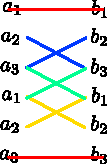
\includegraphics[width=0.2\linewidth]{figures/Kreuzprodukt.pdf} % Pfad anpassen
        \end{figure}
    }

    \begin{equation*}
        \vec{n}\perp\vec{a},\vec{b}\qquad\vec{n}=\text{Normalenvektor}
    \end{equation*}
}

\boxx{Lagebeziehungen}{
    \begin{equation*}
        x=y = \begin{matrix}\text{\rom{1}}\\\text{\rom{2}}\\\text{\rom{3}}\end{matrix}\Bigg|\begin{matrix}x_1=y_1\\x_2=y_2\\x_3=y_3\end{matrix}\Bigg|
    \end{equation*}
    \begin{tabularx}{\textwidth}{>{\centering\arraybackslash}X|>{\centering\arraybackslash}X|>{\centering\arraybackslash}X|>{\centering\arraybackslash}X}
        Lagebeziehung & keine Lösung & eine Lösung & unendlich viele Lösungen\\
        \hline
        Gerade:Gerade & echt Parallel & Schnittpunkt & identisch ($g_1=g_2$)\\
        Gerade:Ebene & echt Parallel & Schnittpunkt & identisch ($g\in E$)\\
        Ebene:Ebene & echt Parallel & Schnittgerade & identisch ($E_1=E_2$)\
    \end{tabularx}
}

\boxx{Schnittwinkel}{
    \begin{tabularx}{\textwidth}{>{\centering\arraybackslash}X|>{\centering\arraybackslash}X|>{\centering\arraybackslash}X}
        Schnittwinkel & trig. & $\alpha$\\
        \hline
        Gerade : Gerade & $\cos(\alpha)=\dfrac{\left|\vec{a}\circ\vec{b}\right|}{\left|\vec{a}\right|\cdot|\vec{b}|}$ & $\alpha=\cos^{-1}\left(\dfrac{\left|\vec{a}\circ\vec{b}\right|}{\left|\vec{a}\right|\cdot|\vec{b}|}\right)$\\
        \hline
        \hline
        Gerade : Ebene & $\cos(\alpha)=\dfrac{\left|\vec{a}\circ\vec{n}\right|}{\left|\vec{a}\right|\cdot|\vec{n}|}$ & $\alpha=\cos^{-1}\left(\dfrac{\left|\vec{a}\circ\vec{n}\right|}{\left|\vec{a}\right|\cdot|\vec{n}|}\right)$\\
        \hline
        \hline
        Ebene : Ebene & $\sin(\alpha)=\dfrac{\left|\vec{n_1}\circ\vec{n_2}\right|}{\left|\vec{n_1}\right|\cdot|\vec{n_2}|}$ & $\alpha=\sin^{-1}\left(\dfrac{\left|\vec{n_1}\circ\vec{n_2}\right|}{\left|\vec{n_1}\right|\cdot|\vec{n_2}|}\right)$
    \end{tabularx}
    \begin{center}
        $\left|\qquad\right|=\text{kleinerer Winkel}$ und $\vec{a},\vec{b}=\text{Richtungsvektoren}$ und $\vec{n}=\text{Normalenvektor}$
    \end{center}
}

\subsection{Geraden}

\boxx{Geradengleichung}{
    \begin{equation*}
        g:\vec{x} = 
        \underbrace{\begin{pmatrix}
        a_1\\
        a_2\\
        a_3
        \end{pmatrix}}_{\text{Stützvektor}}
        +t\cdot 
        \underbrace{\begin{pmatrix}
        b_1\\
        b_2\\
        b_3
        \end{pmatrix}}_{\text{Richtungsvektor}}
    \qquad\qquad t \in \mathbb{R}
    \end{equation*}
}

\boxx{Lagebeziehung}{
    \begin{figure}[H] % Verhindert Gleitverhalten
        \centering
        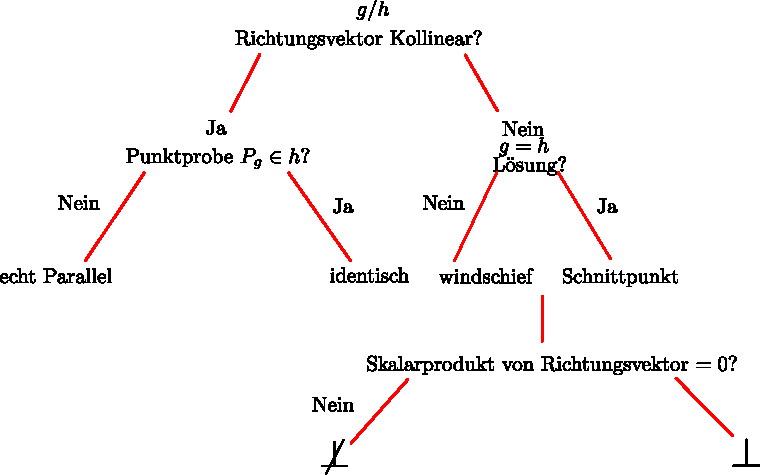
\includegraphics[width=0.8\linewidth]{figures/Lagebeziehung.pdf} % Pfad anpassen
    \end{figure}
}

\boxx{Abstand Gerade:Gerade}{
    \begin{align*}
        g:\vec{x}&=\vec{p}+t\cdot\vec{u} &h:\vec{x}=\vec{q}+s\cdot\vec{v}\\
        \vec{u}&\times\vec{v}=\vec{n} &E\in g
    \end{align*}
    \begin{center}
        $E$ mit $\vec{n}$ aufstellen\\
        $p$ in $E$ einsetzen und d (Koordinatenform) bestimmen
    \end{center}
    \begin{equation*}
        \text{neue Gerade: }\vec{x}=\vec{q}+r\cdot\vec{n}
    \end{equation*}
    \begin{center}
        $\left|\vec{FQ}\right|$ bestimmen
    \end{center}
}


\boxx{Abstand (Lotfußpunkt) Gerade:Punkt}{
    \minipagee{0.5}{
        \begin{center}
            $E=$ Hilfsebene, $g=$ Gerade, $A=$ Punkt
        \end{center}
        \begin{equation*}
            E:\vec{x}=n_1x_1+n_2x_2+n_3x_3=d,\quad\vec{n}=RV\text{ von }g
        \end{equation*}
        \begin{center}
            $A$ in $E$ einsetzen und d berechnen
        \end{center}
        \begin{center}
            $g$ in $E$ einsetzen und $t$ berechnen
        \end{center}
    }
    \minipagee{0.5}{
        \begin{center}
            Orthogonalität: $g:\vec{x}=\underbrace{\begin{pmatrix}c_1\\c_2\\c_3\end{pmatrix}}_{\text{Punkt A}}+t\cdot\begin{pmatrix}b_1\\b_2\\b_3\end{pmatrix}\qquad t\in\mathbb{R}$
        \end{center}
        \begin{equation*}
            \vec{F}=\begin{pmatrix}
                c_1+b_1\cdot t\\
                c_2+b_2\cdot t\\
                c_3+b_3\cdot t
            \end{pmatrix}
        \end{equation*}
        \begin{equation*}
            \vec{AF}\circ\vec{RV}=0
        \end{equation*}
        \begin{equation*}
            \left(c_1+b_1\cdot t\right)\cdot{RV}_1+\left(c_2+b_2\cdot t\right)\cdot{RV}_2+\left(c_3+b_3\cdot t\right)\cdot{RV}_3
        \end{equation*}
        \begin{center}
            $t$ berechnen\\
            $t$ in $g$ einsetzen und $F$ bestimmen
        \end{center}
        \begin{equation*}
            \left|\vec{AF}\right|=\text{kleinster Abstand}
        \end{equation*}
    }
}

\subsection{Ebenen}

\minipagee{0.5}{\boxx{Parameterform}{
    \begin{equation*}
        E:\vec{x}=\underbrace{\begin{pmatrix}
            a_1\\
            a_2\\
            a_3
        \end{pmatrix}}_{\text{Stützvektor}}+r\cdot\underbrace{\begin{pmatrix}
            b_1\\
            b_2\\
            b_3
        \end{pmatrix}}_{\text{Spannvektor}}+s\cdot\underbrace{\begin{pmatrix}
            c_1\\
            c_2\\
            c_3
        \end{pmatrix}}_{\text{Spannvektor}}
    \end{equation*}
}}
\minipagee{0.5}{\boxx{Begrenzung von Ebenen}{
    \begin{center}
        \begin{tikzpicture}[scale=0.5]
            \begin{axis}[
                xlabel={$SV_2$}, ylabel={$SV_1$},
                ticks=none,
                xmin=0, xmax=5, ymin=0, ymax=5, axis lines=middle,
                ]
                \draw[crimson,dashed] (0,5) -- (5,0);
                \draw[jade,thick,dashed] (0,5) -- (5,5) -- (5,0);
            \end{axis}
        \end{tikzpicture}
    \end{center}
    \vspace{-\baselineskip}
    \begin{align*}
        &\crimson{r+s\leq 1}\quad r,s\in\mathbb{R}^+\\
        &\jade{0\leq r,s\leq 1}
    \end{align*}
}}

\boxx{Koordinatenform}{
    \begin{equation*}
        E:ax_1+bx_2+cx_3=d,\quad\begin{pmatrix}
            a\\
            b\\
            c
        \end{pmatrix}=\vec{n}\quad(\text{Kreuzprodukt beider Spannvektoren})
    \end{equation*}
    \begin{center}
        Für $d$ einen Punkt in die Ebene einsetzen
    \end{center}
}

\boxx{Hesse'sche Normalform}{
    \begin{equation*}
        E:\left(\vec{x}-\vec{p}\right)\cdot\vec{n_0}=0
    \end{equation*}
    \begin{center}
        Wobei $\left(\vec{x}-\vec{p}\right)$ ein Verbindungsvektor zwischen zwei Punkten auf der Ebene, und $\vec{n_0}$ der normierte Normalenvektor ist
    \end{center}
    \begin{center}
        Einen Vektoren normiert man, indem man ihn durch seine Länge teilt. Dadurch wird nur noch seine Richtung angegeben:
    \end{center}
    \begin{equation*}
        \vec{n_0}=\dfrac{1}{|\vec{n}|}\cdot\vec{n}
    \end{equation*}

    \boxxline

    \begin{center}
        \jade{Abstand Punkt:Ebene}
    \end{center}
    \begin{equation*}
        \text{Abstand}=\dfrac{ax_1+bx_2+cx_3-d}{\vec{n}}
    \end{equation*}
}



\boxx{Abstand Ebene:Punkt}{
    \begin{center}
        $\vec{n}$ von $E$ bilden
    \end{center}
    \begin{center}
        neue Gerade $g$ mit $\vec{n}$ und Punkt $P$ als Stützvektor
    \end{center}
    \begin{center}
        $E=g\to$ Schnittpunkt $F$
    \end{center}
    \begin{center}
        $\left|\vec{FP}\right|=\text{Abstand}$
    \end{center}
}

\boxx{Abstand Ebene:Gerade}{
    \begin{center}
        $P\in g\to$ Abstand Ebene:Punkt
    \end{center}
}

\boxx{Abstand Ebene:Ebene}{
    \begin{center}
        $P\in E\to$ Abstand Ebene:Punkt
    \end{center}
}
